\section{Creating an Example Project}
\label{sec:example_project}

This section will take you through how to set up a project, create a simple design, run a
simulation, create a top-level design, synthesize and implement your design, and finally
program the FPGA.

Open Vivado, and select File$\rightarrow$New Project or click on Create New Project in the
quick start screen.

\begin{center}
    \begin{tikzpicture}[arrow/.style={-latex, line width=10pt, darkred!70}]
    \node[anchor=south west,inner sep=0] (image) at (0,0)
    {
        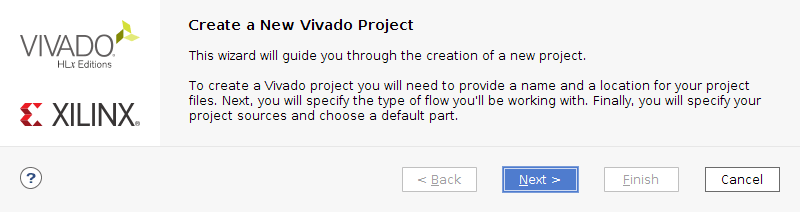
\includegraphics[width=\textwidth]{new_project_start_page}
    };
    \begin{scope}[x={(image.south east)},y={(image.north west)}]
        \node (start) at (0.68,0.64) {};
        \node [below of=start, yshift=-1.2cm] (end) {};
        \draw [arrow] (start) -- node [midway, black] {1} (end);
    \end{scope}
    \end{tikzpicture}

    \begin{tikzpicture}[arrow/.style={-latex, line width=10pt, darkred!70}]
    \node[anchor=south west,inner sep=0] (image) at (0,0)
    {
        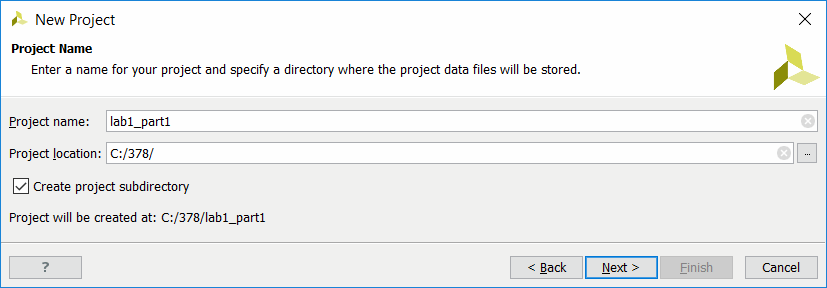
\includegraphics[width=\textwidth]{new_project_name_page}
    };
    \begin{scope}[x={(image.south east)},y={(image.north west)}]
        \node (start) at (0.42,0.58) {};
        \node [left of=start, xshift=-1.2cm] (end) {};
        \draw [arrow] (start) -- node [midway, black] {1} (end);

        \node (start) at (0.38,0.459) {};
        \node [left of=start, xshift=-1.2cm] (end) {};
        \draw [arrow] (start) -- node [midway, black] {2} (end);

        \node (start) at (0.675,0.5) {};
        \node [below of=start, yshift=-1.2cm] (end) {};
        \draw [arrow] (start) -- node [midway, black] {3} (end);
    \end{scope}
    \end{tikzpicture}

    \begin{tikzpicture}[arrow/.style={-latex, line width=10pt, darkred!70}]
    \node[anchor=south west,inner sep=0] (image) at (0,0)
    {
        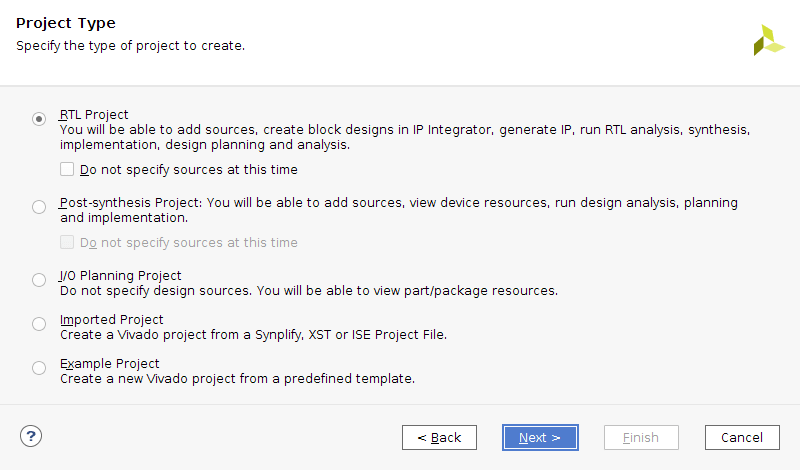
\includegraphics[width=\textwidth]{new_project_type}
    };
    \begin{scope}[x={(image.south east)},y={(image.north west)}]
        %\draw[help lines,xstep=.1,ystep=.1] (0,0) grid (1,1);
        \node (start) at (0.672,0.3) {};
        \node [below of=start, yshift=-1.2cm] (end) {};
        \draw [arrow] (start) -- node [midway, black] {} (end);
    \end{scope}
    \end{tikzpicture}
\end{center}

Make sure the "Target language" is set to VHDL.
Then create two source files, gates2 and gates2\_tb.
You can skip adding any files during project creation in the future, but for now to show how
this is done we will do it here.

\begin{center}
    \begin{tikzpicture}[arrow/.style={-latex, line width=10pt, darkred!70}]
    \node[anchor=south west,inner sep=0] (image) at (0,0)
    {
        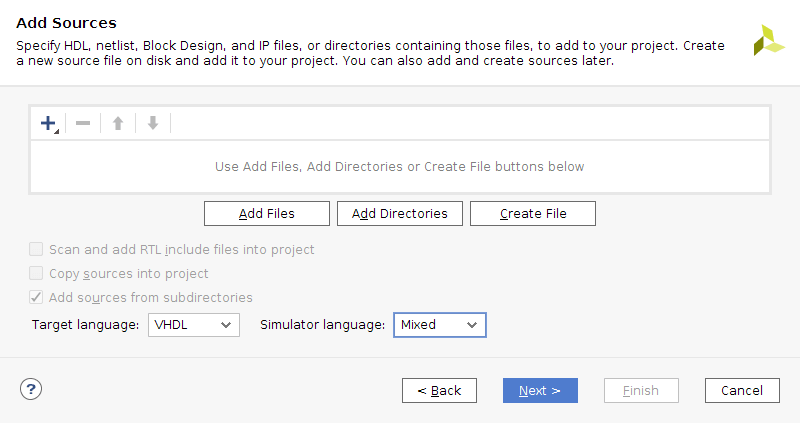
\includegraphics[width=\textwidth]{new_project_add_sources}
    };
    \begin{scope}[x={(image.south east)},y={(image.north west)}]
        \node (start) at (0.42,0.23) {};
        \node [left of=start, xshift=-1.2cm] (end) {};
        \draw [arrow] (start) -- node [midway, black] {1} (end);

        \node (start) at (0.85,0.495) {};
        \node [left of=start, xshift=-1.2cm] (end) {};
        \draw [arrow] (start) -- node [midway, black] {2} (end);
    \end{scope}
    \end{tikzpicture}

    \begin{minipage}[b]{0.49\textwidth}
        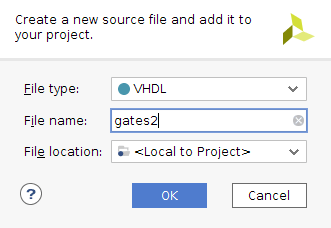
\includegraphics[width=\textwidth]{create_gates2}
    \end{minipage}
    \hfill
    \begin{minipage}[b]{0.49\textwidth}
        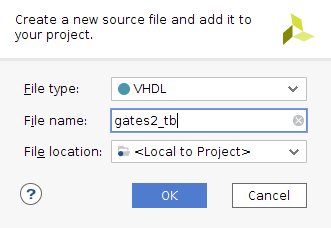
\includegraphics[width=\textwidth]{create_gates2_tb}
    \end{minipage}
\end{center}

After creating gates2\_tb, set it to simulation only.
We will create a testbench with this file which only gets used in simulation.
Now you should have the following showing:

\begin{center}
    \begin{tikzpicture}[arrow/.style={-latex, line width=10pt, darkred!70}]
    \node[anchor=south west,inner sep=0] (image) at (0,0)
    {
        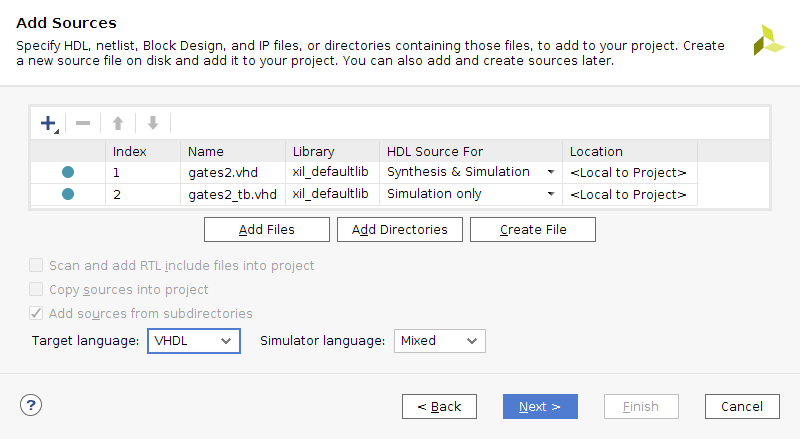
\includegraphics[width=\textwidth]{new_project_sources_added}
    };
    \begin{scope}[x={(image.south east)},y={(image.north west)}]
        \node (start) at (0.8,0.555) {};
        \node [left of=start, xshift=-1.2cm] (end) {};
        \draw [arrow] (start) -- node [midway, black] {1} (end);

        \node (start) at (0.675,0.32) {};
        \node [below of=start, yshift=-1.2cm] (end) {};
        \draw [arrow] (start) -- node [midway, black] {2} (end);
    \end{scope}
    \end{tikzpicture}
\end{center}

Now find the proper Xilinx Design Constraints (XDC) file for your board.
For Dr. Hanna or Dr. Gorski's class you should use one provided on Moodle which offer
preconfigured names for outputs matching the book's examples.
For Dr. LLamocca's class you should use the master XDC file provided by Digilent Inc.
He has made it available on Moodle as well.
Make sure you use the correct XDC file for your board, and note that the Nexys 4 and Nexys 4 DDR
are two different boards.

Check "Copy constraints files into project" to copy the .xdc file into the project folder.
Otherwise, the .xdc file will be linked to and if you ever move or delete it your project
will no longer work.

\begin{center}
    \begin{tikzpicture}[arrow/.style={-latex, line width=10pt, darkred!70}]
    \node[anchor=south west,inner sep=0] (image) at (0,0)
    {
        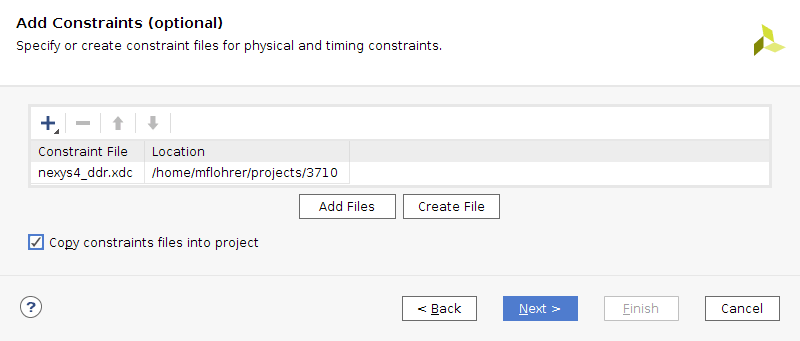
\includegraphics[width=\textwidth]{new_project_add_constraints}
    };
    \begin{scope}[x={(image.south east)},y={(image.north west)}]
        \node (start) at (0.61,0.393) {};
        \node [left of=start, xshift=-1.2cm] (end) {};
        \draw [arrow] (start) -- node [midway, black] {1} (end);

        \node (start) at (0.45,0.286) {};
        \node [left of=start, xshift=-1.2cm] (end) {};
        \draw [arrow] (start) -- node [midway, black] {2} (end);

        \node (start) at (0.676,0.42) {};
        \node [below of=start, yshift=-1.2cm] (end) {};
        \draw [arrow] (start) -- node [midway, black] {3} (end);
    \end{scope}
    \end{tikzpicture}
\end{center}

On the next screen you pick the FPGA that we are targeting, in the case of the Nexys 4 or
Nexys 4 DDR board it is an Artix 7 with part number xc7a100tcsg324-1.
The Basys 3 has an Artix 7 FPGA with part number xc7a35tcpg236-1.
You can use the filter categories and search box to limit the selection to the desired part number.

\begin{center}
    \begin{tikzpicture}[arrow/.style={-latex, line width=10pt, darkred!70}]
    \node[anchor=south west,inner sep=0] (image) at (0,0)
    {
        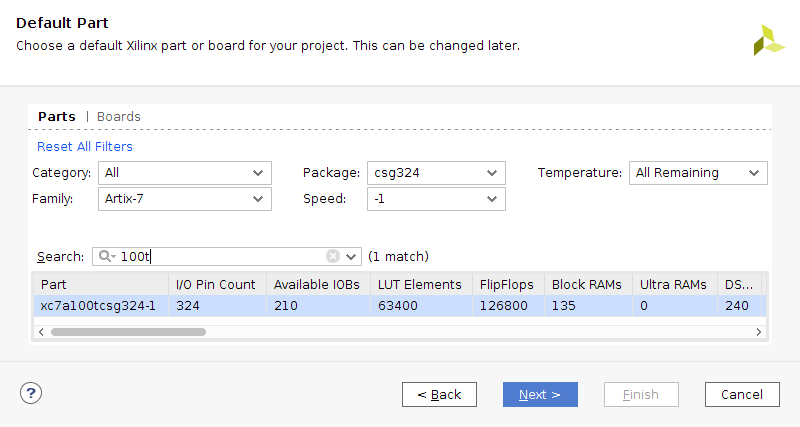
\includegraphics[width=\textwidth]{new_project_part}
    };
    \begin{scope}[x={(image.south east)},y={(image.north west)}]
        \node (start) at (0.61,0.393) {};
        \node [left of=start, xshift=-1.2cm] (end) {};
        \draw [arrow] (start) -- node [midway, black] {1} (end);

        \node (start) at (0.676,0.3) {};
        \node [below of=start, yshift=-1.2cm] (end) {};
        \draw [arrow] (start) -- node [midway, black] {2} (end);
    \end{scope}
    \end{tikzpicture}
\end{center}

To finish the project creation step make sure the summary looks correct and then press Finish.

\begin{center}
    \begin{tikzpicture}[arrow/.style={-latex, line width=10pt, darkred!70}]
    \node[anchor=south west,inner sep=0] (image) at (0,0)
    {
        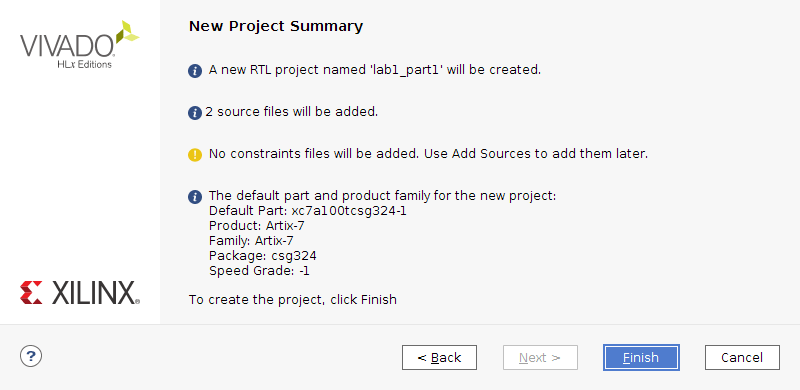
\includegraphics[width=\textwidth]{new_project_summary}
    };
    \begin{scope}[x={(image.south east)},y={(image.north west)}]
        \node (start) at (0.8,0.35) {};
        \node [below of=start, yshift=-1.2cm] (end) {};
        \draw [arrow] (start) -- node [midway, black] {} (end);
    \end{scope}
    \end{tikzpicture}
\end{center}

Since you listed two files to create, after creating the project a window will pop-up asking to
define the inputs and outputs of the two files.
They should be exactly as shown below, gates2\_tb has no inputs or outputs, and gates2 has a and b
as inputs and a 6-bit bus z[5:0] as an output.

\begin{center}
    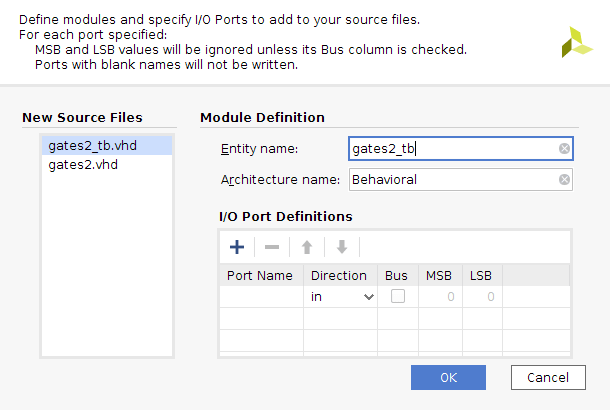
\includegraphics[width=\textwidth]{define_modules_gates2}
    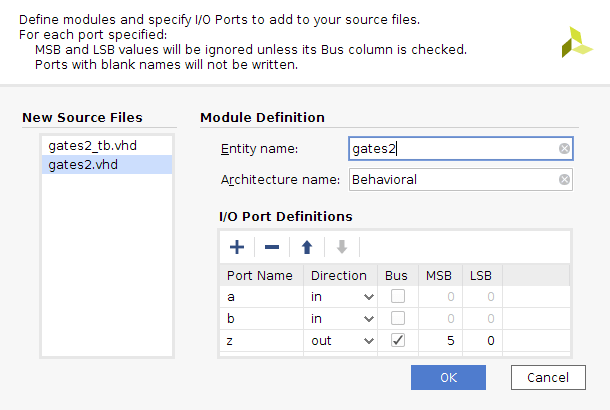
\includegraphics[width=\textwidth]{define_modules_gates2_tb}
\end{center}

Once you press OK, you should see the following screen, other than some extra sections that are
minimized so that the screenshots fit in this document easier.
On the left is your sources list, which have all your project files listed.
If you click on gates2, it will open it in the right section and you will see the auto-generated
code skeleton.
You should see your a, b, and z signals you created earlier as inputs and outputs to the module.

\begin{center}
    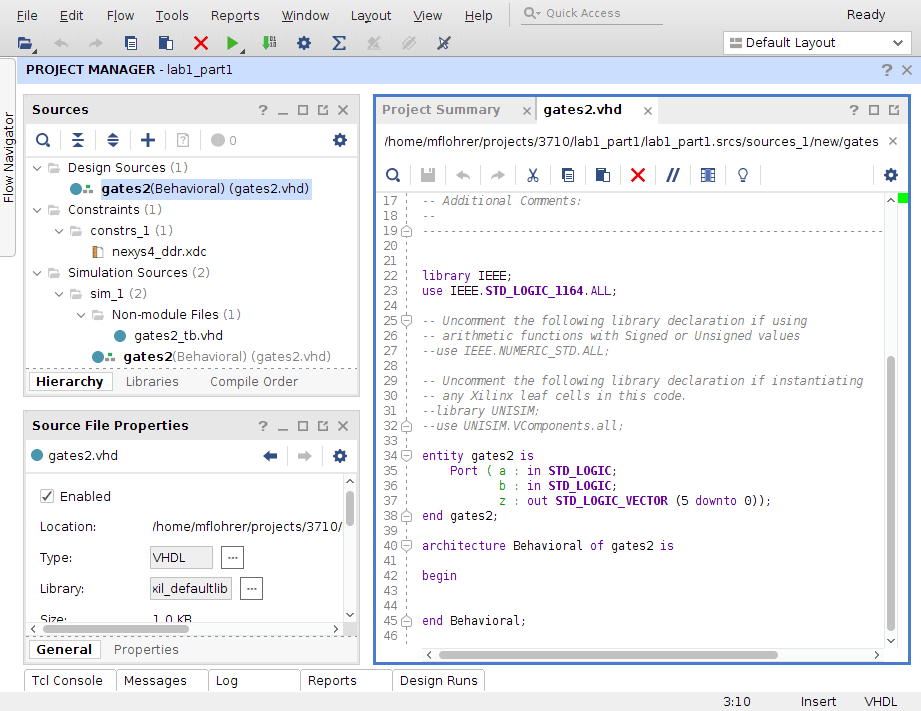
\includegraphics[width=\textwidth]{project_gates2}
\end{center}

Edit the file so that is looks like the following picture.
Alternatively, easy to copy code is given below.
Note that all the auto-generated comments were removed, feel free to leave or remove them as
you wish, or even add your own comments! It is a good idea to add your name and date at the top
of the file in a comment.

\begin{lstlisting}[language=VHDL]
z(5) <= a and b;
z(4) <= a nand b;
z(3) <= a or b;
z(2) <= a nor b;
z(1) <= a xor b;
z(0) <= a xnor b;
\end{lstlisting}

\begin{mdframed}[style=note]
    VHDL is case-insensitive. Capital letters don't matter.
\end{mdframed}

\begin{center}
    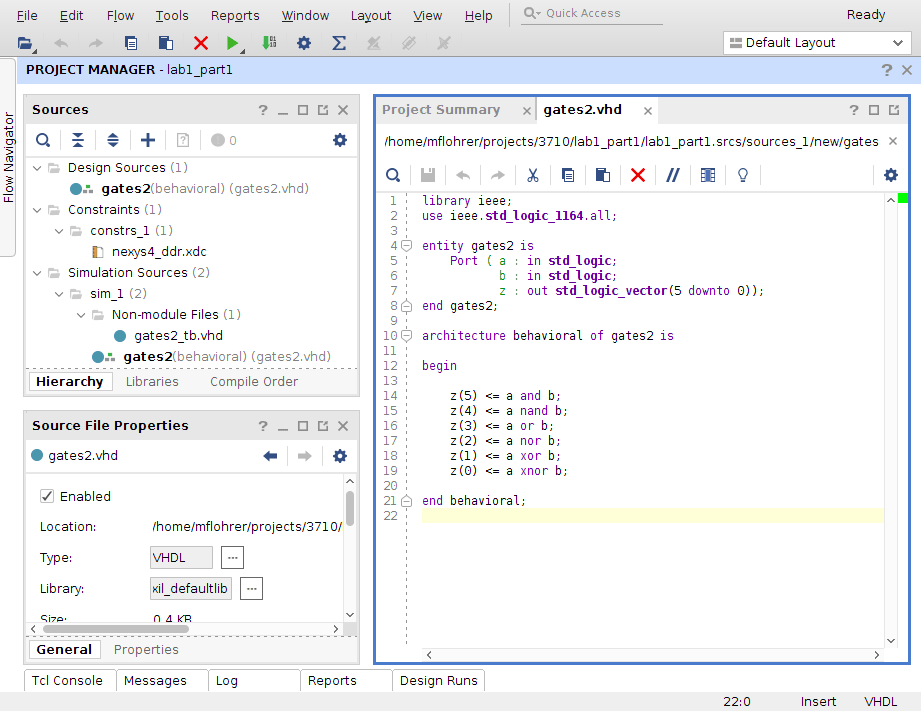
\includegraphics[width=\textwidth]{project_gates2_modified}
\end{center}

Vivado seems to sometimes have a bug when creating simulation-only sources like our gates2\_tb.
It sometimes creates a blank file under the simulation directory and also a skeleton VHDL file
under the source directory.
The picture below on the left shows the project directory structure and the two gates2\_tb.vhd
files that were created.
To fix this bug after creating a simulation-only source, move the file under the source directory
to replace the one in the simulation directory.
When done the project directory should look like the picture below on the right.

\vspace{3mm}
\noindent
\begin{minipage}[b]{0.45\textwidth}
    \centering
    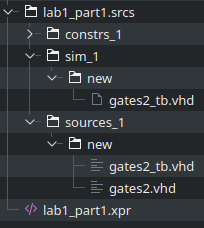
\includegraphics[width=0.7\textwidth]{testbench_sources_bug}
\end{minipage}
\hfill
\begin{minipage}[b]{0.45\textwidth}
    \centering
    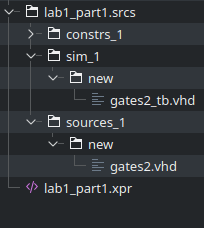
\includegraphics[width=0.7\textwidth]{testbench_sources_bug_fixed}
\end{minipage}
\vspace{1mm}

Back in Vivado, since the testbench file, gates2\_tb was created as simulation-only,
it will show up under the simulation sources section.
Click on it to open it and modify it to have the following code.

\noindent
\begin{minipage}{\textwidth}
\begin{verbatim}
library ieee;
use ieee.std_logic_1164.all;

entity gates2_tb is
end gates2_tb;

architecture behavioral of gates2_tb is
    component gates2
    port( a : in  std_logic;
          b : in  std_logic;
          z : out std_logic_vector(5 downto 0)
        );
    end component;
    -- Inputs
    signal a : std_logic := '0';
    signal b : std_logic := '0';
    -- Outputs
    signal z : std_logic_vector(5 downto 0);
begin
    -- Instantiate the Unit Under Test (UUT)
    uut: gates2 port map (
            a => a,
            b => b,
            z => z
        );
    -- Stimulus process
    stim_proc: process
    begin
        a <= '0';
        b <= '0';
        wait for 20 ns;

        a <= '0';
        b <= '1';
        wait for 20 ns;

        a <= '1';
        b <= '0';
        wait for 20 ns;

        a <= '1';
        b <= '1';
        wait for 20 ns;

        wait;
    end process;
end behavioral;
\end{verbatim}
\end{minipage}
\strut

Once you are done run a behavioral simulation by clicking on Run Simulation and then Run
Behavioral simulation in the Flow Navigator to the left.
Make sure to save your files after you are done editing them, Vivado does not save files
automatically before running the simulation.

\begin{center}
    \begin{tikzpicture}[arrow/.style={-latex, line width=10pt, darkred!70}]
    \node[anchor=south west,inner sep=0] (image) at (0,0)
    {
        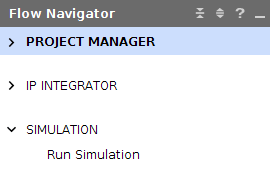
\includegraphics{project_flow_simulation}
    };
    \begin{scope}[x={(image.south east)},y={(image.north west)}]
        \node (start) at (0.83,0.1) {};
        \node [left of=start, xshift=-1.2cm] (end) {};
        \draw [arrow] (start) -- node [midway, black] {} (end);
    \end{scope}
    \end{tikzpicture}
\end{center}

When the simulation runs, you will want to press zoom-fit so that you can see the entire
simulation.
However, by default the simulation runs for 1 μs which happened to be longer than needed in
this case.
All the action happened in the first 100 ns!

\begin{center}
    \begin{tikzpicture}[arrow/.style={-latex, line width=10pt, darkred!70}]
    \node[anchor=south west,inner sep=0] (image) at (0,0)
    {
        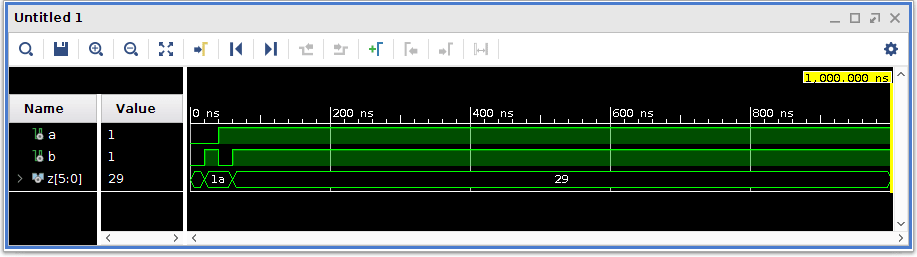
\includegraphics[width=\textwidth]{simulation_zoom_fit}
    };
    \begin{scope}[x={(image.south east)},y={(image.north west)}]
        \node (start) at (0.32,0.81) {};
        \node [left of=start, xshift=-1.2cm] (end) {};
        \draw [arrow] (start) -- node [midway, black] {} (end);
    \end{scope}
    \end{tikzpicture}
\end{center}

Zoom in to the first 100 ns by clicking the zoom in button and dragging the scrollbar.
Alternatively, you can click and hold the mouse to zoom in, out, fit, or to a range.
When you zoom in, it zooms at the location of the cursor.
You can click on the waveform to put the cursor at that location.

\begin{center}
    \begin{tikzpicture}[arrow/.style={-latex, line width=10pt, darkred!70}]
    \node[anchor=south west,inner sep=0] (image) at (0,0)
    {
        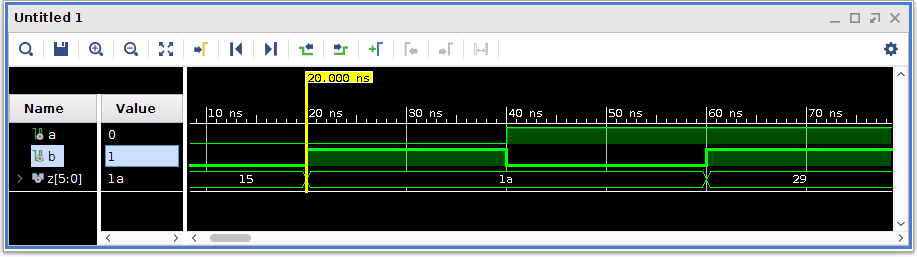
\includegraphics[width=\textwidth]{simulation_zoomed}
    };
    \begin{scope}[x={(image.south east)},y={(image.north west)}]
        \node (start) at (0.24,0.81) {};
        \node [left of=start, xshift=-1.2cm] (end) {};
        \draw [arrow] (start) -- node [midway, black] {} (end);
    \end{scope}
    \end{tikzpicture}
\end{center}

You can see from time 0-20 ns that the inputs a and b are both 0, so the output should be 0x15.
You can check the truth tables of all the gates to see that this is correct.
Then the rest of the truth table is simulated in the simulation.
If your simulation doesn't look correct, go back and check your code to make sure it is correct.
Once the simulation is correct, we can add the top-level file that will connect the inputs and
outputs to some physical things on the board like switches and LEDs.

% FIGS

Just like in the testbench, in the top-level we are going to port-map in the gates2 component.
We will simply wire up the I/O of gates2 to the switches and LEDs.
Type in the following code so that your gates2\_top looks like the following picture.

% FIGS

Now we need pin constraints.
These will map our top-level inputs and outputs, for this example sw[1:0] and ld[5:0] to the
physical pins on the FPGA so that they are connected to the external switches and LEDs.
We have preconfigured the constraints file for you, so all you have to do is download it from
Moodle and add it to your project.

% FIGS

Now that the constraints have been added, we can generate the .bit file that will be
programmed to the FPGA.
The steps that are required are to run Synthesis, Implementation, and then Generate Bitstream.
However, as a shortcut, you can click on Generate Bitstream and it will automatically run the
other steps if they need to be run.

% FIGS
Open target$\rightarrow$Auto connect
Program device$\rightarrow$xc7a100t\_0
% FIGS


